
\usetikzlibrary{decorations.pathmorphing}
\usetikzlibrary{decorations.markings}
\usetikzlibrary{decorations.pathmorphing}
\usetikzlibrary{arrows}
\usetikzlibrary{automata}
\usetikzlibrary{patterns}
\usetikzlibrary{shapes}
\usetikzlibrary{calc}


\newlength{\hatchspread}
\newlength{\hatchthickness}
\newlength{\hatchshift}
\newcommand{\hatchcolor}{}
% declaring the keys in tikz
\tikzset{hatchspread/.code={\setlength{\hatchspread}{#1}},
         hatchthickness/.code={\setlength{\hatchthickness}{#1}},
         hatchshift/.code={\setlength{\hatchshift}{#1}},% must be >= 0
         hatchcolor/.code={\renewcommand{\hatchcolor}{#1}}}
% setting the default values
\tikzset{hatchspread=3.5pt,
         hatchthickness=0.5pt,
         hatchshift= 2pt,% must be >= 0
         hatchcolor=black!90}
% declaring the pattern
\pgfdeclarepatternformonly[\hatchspread,\hatchthickness,\hatchshift,\hatchcolor]% variables
   {custom north west lines}% name
   {\pgfqpoint{\dimexpr-2\hatchthickness}{\dimexpr-2\hatchthickness}}% lower left corner
   {\pgfqpoint{\dimexpr\hatchspread+2\hatchthickness}{\dimexpr\hatchspread+2\hatchthickness}}% upper right corner
   {\pgfqpoint{\dimexpr\hatchspread}{\dimexpr\hatchspread}}% tile size
   {% shape description
    \pgfsetlinewidth{\hatchthickness}
    \pgfpathmoveto{\pgfqpoint{0pt}{\dimexpr\hatchspread+\hatchshift}}
    \pgfpathlineto{\pgfqpoint{\dimexpr\hatchspread+0.15pt+\hatchshift}{-0.15pt}}
    \ifdim \hatchshift > 0pt
      \pgfpathmoveto{\pgfqpoint{0pt}{\hatchshift}}
      \pgfpathlineto{\pgfqpoint{\dimexpr0.15pt+\hatchshift}{-0.15pt}}
    \fi
    \pgfsetstrokecolor{\hatchcolor}
%    \pgfsetdash{{1pt}{1pt}}{0pt}% dashing cannot work correctly in all situation this way
    \pgfusepath{stroke}
   }

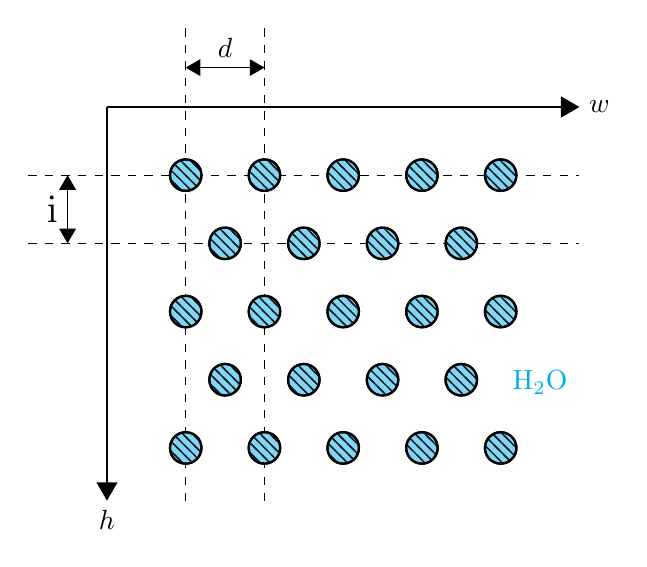
\begin{tikzpicture}[>=triangle 60]

%axis
\def\r{0.866025403784439}
\coordinate (o) at (0,0);
\coordinate (x) at (6,0);
\coordinate (y) at (0,-5);

\draw[thick,->] (o)--(x); 
\draw[thick,->] (o)--(y); 

\node [anchor=west] at (x) {$w$}; 
\node [anchor=north] at (y) {$h$}; 

% dashed lines
%vertical
\draw[dashed] (1,1)--(1,-5);
\draw[dashed] (2,1)--(2,-5);

%horizontal
\draw[dashed] (-1,-\r)--(6,-\r);
\draw[dashed] (-1,-2*\r)--(6,-2*\r);

%arrow and quotes

%vertical
\draw[->] (-0.5,-1.5*\r)--(-0.5,-\r);
\draw[->] (-0.5,-1.5*\r)--(-0.5,-2*\r);
\node [anchor=east] at (-0.5,-1.5*\r) {\Large i}; 

%horizontal
\draw[->] (1.5,0.5)--(1,0.5);
\draw[->] (1.5,0.5)--(2,0.5);
\node [anchor=south] at (1.5,0.5) {$d$}; 


%\node [color=cyan,anchor=center] at (5.5,-3.5) { \contour{black}{\textcolor{cyan}{H$_2$O}} }; 
\node [color=cyan,anchor=center] at (5.5,-3.5) {H$_2$O}; 
%tubes
\foreach \x in {1,...,5}
{
    \foreach \j in {-1,...,-3}
    {
    		\draw[thick,fill=cyan!50] (\x,\j*\r*2+\r) circle(0.2);
    		\draw[thick,pattern=custom north west lines] (\x,\j*\r*2+\r) circle(0.2);
    }
}

\foreach \x in {1.5,...,4.5}
{
    \foreach \j in {-1,...,-2}
    {
    		\draw[thick,fill=cyan!50] (\x,\j*\r*2) circle(0.2);
    		\draw[thick,pattern=custom north west lines] (\x,\j*\r*2) circle(0.2);
    }
}


%fill
%\draw[fill=cyan!50,even odd rule] (0,-1) arc (-90:90:2);


%\draw[pattern=custom north west lines, pattern color=black, even odd rule] (0,-1) arc (-90:90:2) (0,-2) arc (-90:90:3); 

%\draw[fill=black!40, even odd rule] (0,-2) arc (-90:90:3) (0,-3) arc (-90:90:4); 

%\draw[fill=blue!40,draw=white!0, even odd rule] (0,-3) arc (-90:90:4) rectangle (0,-4)--(0,6)--(6,6)--(6,-4); 

%contour
%\draw[thick] (0,-1) arc (-90:90:2); 

%resistor symbol


%\draw[*-*,very thick, decorate,decoration=zigzag] (a)--(b);

% names

%\node [anchor=center] at (0.7,0.2) {\Large H$_2$O}; 

%\node [anchor=west,align=center] at (3.6,-2.1) {\Large Stainless\\ \Large steel}; 

\end{tikzpicture}